\chapter{Desenvolvimento da RNA}
\label{chp:criacaoRNAs}

Uma vez que a fase de pré processamento do dataset foi implementada com funções auxiliares desenvolvidas em \textit{Python}, para a frase de desenvolvimento da RNA manteve-se a mesma linguagem de programação. Assim, alem de se manter o mesmo ambiente de desenvolvimento, \textit{Python} disponibiliza as principais APIs de criação de RNAs atualmente utilizadas. 

Como plataforma escolhida para executar a rede, foi utilizada a ferramenta \textit{Keras}. 
Esta ferramenta apresenta um conjunto de características que se adequam com o contexto deste projeto, nomeadamente: 
\begin{itemize}
    \item É bastante simples de usar, permitindo rapidamente obter uma estrutura de rede capaz de analisar os dados. 
    
    Contudo, permite também evoluir a rede a nível de complexidade, interligando com outras plataformas de criação de RNAs (\textit{TensorFlow, Theano, CNTK}) e permitindo ainda alterar o contexto de execução da RNA (CPU ou GPU);
    
    \item Devido ao volume do dataset apresentar mais de 900 mil instâncias, alimentar a rede com todos os dados numa fase de treino única exigia recursos e uma capacidade de processamento continua durante demasiado tempo. 
    
    Contudo, os métodos da plataforma \textit{Keras} permitem criar várias fases de treino, que evoluem a rede face ao estado de treino anterior. Desta forma é possível dividir o dataset em subconjuntos que são utilizados em fases de treino iterativas, exigindo assim menores recursos de memória e tempo de processamento na fase de aprendizagem;
    
    \item Pelo mesmo motivo do tópico anterior, treinar a rede sempre que for necessário realizar algum tipo de previsão não é viável em problemas com um elevado número de dados. 
    
    Como solução, \textit{Keras} disponibiliza funções para guardar o estado da RNA. É assim possível armazenar tanto a arquitetura, como os pesos das ligações dos axónios, após uma fase de treino ou teste da rede;
    
    \item \textit{Keras} permite parametrizar praticamente todos os aspetos relacionados com a topologia da rede, como o número de camadas; ligações entre camadas; funções de ativação por camada; métricas de avaliação interna da rede e o \textit{optimizer} (método de aprendizagem da rede). 
\end{itemize}

Tendo por base a experiência anterior com outras plataformas de desenvolvimento de RNAs, como \textit{R, Julia ou MXNet}, a plataforma \textit{Keras} apresenta-se como a mais indicada e modular para este contexto.
Focando o conjunto de motivos anterior e sendo atualmente uma plataforma bastante utilizada para a criação de RNAs, a plataforma \textit{Keras} foi assim a escolhida para o desenvolvimento da rede deste projeto. 


\section{Representação Texto \textit{Input} - Matrizes One-Hot}
\label{sec:vectPalavras}

Uma das decisões essenciais do uso de RNAs num problema de classificação de texto, passa por codificar as palavras/frases que compõe o texto num formato que seja capaz de ser analisado e processado corretamente pelos neurónios da rede. 

Devido à natureza da sua implementação, como o caso das funções de ativação que a rede utiliza na fase de aprendizagem, a sua estrutura está preparada para lidar apenas e preferencialmente com dados numéricos. Desta forma, uma palavra no seu formato literal e digital (\textit{Strings}) não são assim formatos indicados para alimentar e treinar uma rede que se procure treinar de forma viável e adequadamente. 

É assim necessário converter as palavras e a estrutura sequencial de uma frase num atributo (ou vários) caracterizado por valores numéricos. 
Encontrar formas de representação/tradução de linguagem natural para modelos de representação úteis em inteligência artificial não se apresenta como uma decisão simples, variando conforme o contexto sobre o qual se procura analisar a frase. 

Os dois procedimentos mais utilizados para representar texto são associados com as estruturas \textit{Vector Embeddings} ou Matrizes \textit{One-Hot}. 
\textit{Embeddings Vectors} são mapeamentos no espaço de palavras e/ou frases, em que a sua localização indica as semelhanças (Figura \ref{fig:vectorEmbeddings}). Esta representação permite ainda associar relações semânticas, através da distancia dos vetores, sendo por isso muito usadas em contextos que envolvem a geração de analogias.

\begin{figure}[H]
    \hspace{-0.2in}
    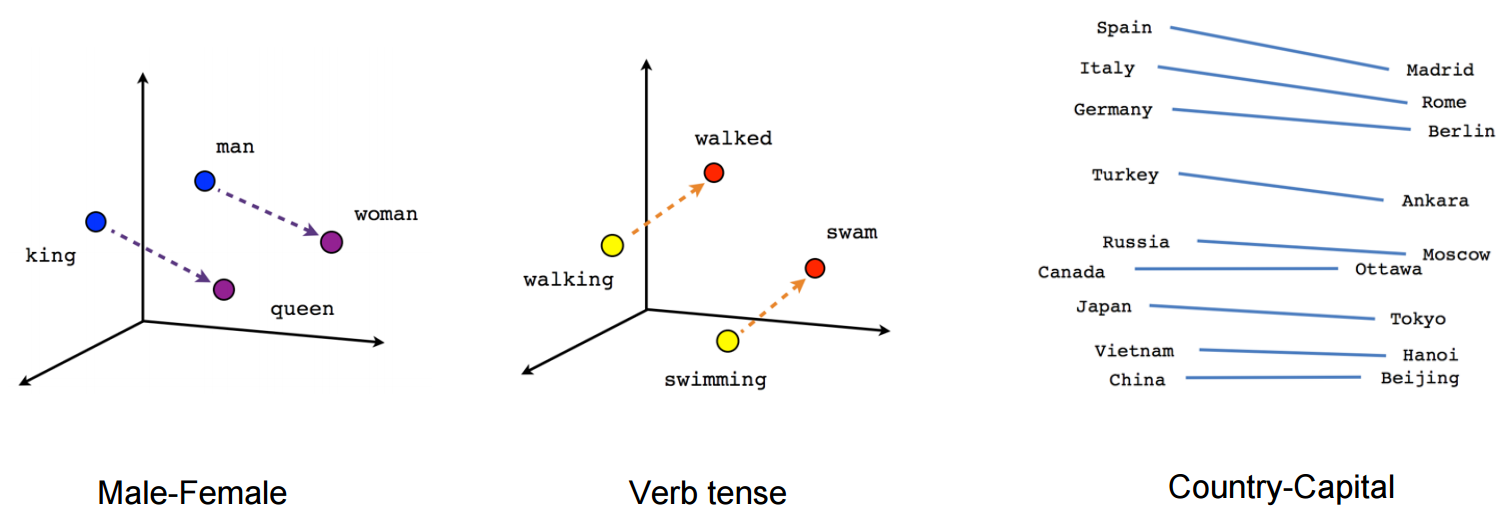
\includegraphics[scale=0.3]{Imagens/vector_embeddings.png}
    \caption{Representação simbólica de \textit{Vector Embeddings}}
    \label{fig:vectorEmbeddings}
\end{figure}


Em oposição, as estruturas matriciais \textit{One-Hot} não contêm informação de relações linguísticas entre as palavras. 
De uma forma geral, permitem apenas saber quais as palavras que surgem num determinado texto, não contendo informações sobre as relações entre as palavras, como a sua ordem ou semelhança na frase.

Para o contexto de classificação emotiva de texto, procura-se exatamente representar as palavras que se encontrem num determinado texto, num formato capaz de ser processado pelas camada de input de uma RNA. Nesse sentido, devido à sua simplicidade, as matrizes One-Hot foram o modelo de representação escolhido. 

Este tipo de matrizes são chamadas de \textit{One-Hot} já que cada matriz tem uma característica distinta ("hot") de todas as outras.

Considerando como exemplos as seguintes frases:
\begin{minted}[tabsize=4, breaklines=true]{text}
            Errors should never pass silently.
            Unless explicitly silenced.
\end{minted}

A representação numa matriz One-Hot das seguintes frases começa por "partir" as frases numa lista (vetor) de palavras, sem ocorrência de repetições. 

\begin{minted}[tabsize=4,breaklines=true]{Python}
    ['errors', 'should', 'never', 'pass', 'silently', 'unless', 'explicitly', 'silenced']
\end{minted}

Depois de criada a lista de palavras únicas no texto a representar, é criado aquilo que pode ser visto como um dicionário com todas as palavras distintas, atribuindo um id único a cada palavra. Neste processo, não é relevante a ordem das palavras. Cada id será apenas um identificador único de cada palavras e irá representar apenas o índice \textit{i,j} da matriz que representa aquela palavra.

\begin{minted}[tabsize=4,breaklines]{Python}
    {
          'errors': 0,      
          'should': 1,
          'never': 2,
          'pass': 3,
          'silently': 4,
          'unless': 5,
          'explicitly': 6,
          'silenced': 7,
    }
\end{minted}

Distribuídos os ids pelas palavras encontradas, a matriz \textit{One-Hot} terá tantas colunas quantas palavras encontradas no texto (dimensão dicionário) e, tantas linhas quantas as palavras encontradas na frase a codificar. 
No exemplo anterior, o dicionário de dados apresenta 8 palavras distintas e a primeira frase 5 palavras. Assim, uma matriz One-Hot que represente esta primeira frase terá dimensões 5x8. 

Em cada linha, o valor 1 no indice i,j que representa a palavra indica a ocorrência da mesma na palavra. Em oposição, o valor 0 indica a não ocorrência da palavra identificada pela linha. 

Para construir estas matrizes foram usados métodos disponibilizados na API \textit{Pre Processing Text} da plataforma \textit{Keras}. Nestas funções, as matrizes One-Hot devolvidas apresentam a vantagem de serem matrizes quadradas, podendo ser facilmente convertidas num vetor de palavras, considenrado apenas os valores da sua diagonal. Deste modo, o valor 1 num determinado indice indica a ocorrência, ou não, daquela palavra no texto representado pelo vetor de palavras. 

\begin{minted}[tabsize=4,breaklines]{Python}
    [
        [1, 0, 0, 0, 0, 0, 0, 0], #errors
        [0, 1, 0, 0, 0, 0, 0, 0], #should
        [0, 0, 1, 0, 0, 0, 0, 0], #never
        [0, 0, 0, 1, 0, 0, 0, 0], #pass
        [0, 0, 0, 0, 1, 0, 0, 0], #silently
        [0, 0, 0, 0, 0, 0, 0, 0], #unless
        [0, 0, 0, 0, 0, 0, 0, 0], #explicitly
        [0, 0, 0, 0, 0, 0, 0, 0], #silenced
    ]
\end{minted}

Na implementação utilizada, utilizaram-se vetores de palavras com 3500 posições, representando assim a 3500 palavras mais utilizadas. 
Infelizmente, apesar desta representação ser bastante simples e eficaz no contexto, implica que as RNAs apresentem tantos nodos de \textit{input} quantos índices do vetor. 

Por este motivo e por questões de memória, para representar em vetores de palavras todos os tweets utilizados na fase de aprendizagem da rede, foram apenas utilizados vetores com 3500 posições. 

\section{Arquitetura da RNA}

Para a definição da topologia da rede neuronal, foi utilizada uma arquitetura multi-layer FeedForward (Secção \ref{sec:Arquiteturas}). Em \textit{Keras} este tipo de rede designa-se como \textit{sequencial} e representa assim uma rede \textit{multi-layer perception}.

A criação de diferentes camadas camadas intermédias recorre ao método \textit{Dense}, que na plataforma caracteriza uma camada de neurónios totalmente conectada com os neurónios da camada anterior. 

\begin{minted}[tabsize=4, breaklines=true]{Python} 
    # Exemplo da Definicao da topologia da rede
    self.model = Sequential()
    self.model.add(Dense(512, input_shape=(self.max_words,), activation='tanh', kernel_initializer="uniform"))
    self.model.add(Dropout(0.5))
    self.model.add(Dense(256, activation='tanh', kernel_initializer="uniform"))
    self.model.add(Dense(128, activation='tanh', kernel_initializer="uniform"))
    self.model.add(Dense(3, activation='tanh'))
\end{minted}

Neste processo de criação de diferentes topologias foram tido alguns cuidados, destacando-se os seguintes aspetos: 

\begin{itemize}
    \item Na primeira camada intermédia, através do parâmetro \textbf{\textit{input\_shape}} a camada identifica automaticamente o número de neurónios da camada de input. 
    Neste caso, existem tantos neurónios de input quantos elementos do vetor de palavras que representa a frase do \textit{Tweet} (Secção \ref{sec:vectPalavras});
    
    \item O argumento \textbf{\textit{activation}} define a função de ativação a utilizar na camada. 

    Muitas das principais funções utilizadas em contextos de RNAs apresentam apenas um contradomínio entre [0,1] ou [0, inf].
    Uma vez que existem três classes target ({Negativo, Neutro, Positivo}), identificadas respetivamente pelos valores {-1, 0, 1}, foi tido o cuidado de utilizar funções de ativação que mantivessem o seu contradomínio entre [-1, 1]. 
    
    Utilizar funções sem contradomínio negativo, reduziria a capacidade de aprendizagem dos casos de publicações com nível emocional negativo. 
    Contudo, como em teoria o processo de aprendizagem é capaz de lidar com nodos que sejam reduzidos ao valor 0, foram também utilizadas algumas funções com contradomínio diferente de [-1, 1]. 
    
    Nomeadamente, foram experimentadas algumas adaptações da função ReLU;
    
    \item O parâmetro \textbf{\textit{Kernel initializer}} define qual o método utilizado para gerar o valor inicial dos pesos das ligações. 
    
    Neste projeto foram exploradas funções como a distribuição normal, uniforme e, maioritariamente, a distribuição de \textit{Xavier} \cite{xavier}.
    
    \item Na tentativa de evitar cenários de overfitting, podem ser adicionadas camadas \textit{Dropout} através de um método com o mesmo nome.
    
    \begin{minted}[tabsize=4, breaklines=true]{Python} 
        # Exemplo da adição de uma dropout layer com probabilidade = 0.2
        self.model.add(Dropout(0.2))
    \end{minted}
    
    O processo de \textit{dropout} acontece apenas na fase de treino e ocorre depois da fase de ativação do neurónio. 
    Esta camada opera de forma aleatória, colocando algumas ativações com o valor zero. Desta forma é simulado o conceito de "esquecimento", descartando alguma informação e "apagando" partes da rede neuronal em algumas iterações. 

    Contudo, estas camadas não devem ser introduzidas logo na fase inicial e foram exploradas apenas em cenários de overfitting ou na tentativa de obter melhores resultados de classificação. 
\end{itemize}

\section{Padrões de Treino}
\label{sec:padroesTreino}

Depois de especificada a arquitetura que dará suporte à representação da rede neuronal, o processo de aprendizagem da rede pode ser dividido em duas etapas: a definição de uma método de aprendizagem, segundo um conjunto de métricas de avaliação e, a fase de análise e generalização efetiva dos dados, realizando o ajustamento dos pesos da rede aos mesmos. 

\subsection{Método de Aprendizagem}

Para definir o comportamento de aprendizagem da rede é utilizado o método \textit{Compile}. 

Na escolha de um optimizador e métricas de avaliação, necessários de fornecer a este método, foram tomadas as seguintes considerações:
\begin{itemize}

    \item O parâmetro \textit{optimizer} define a técnica de aprendizagem utilizada. Neste projeto foi escolhido o método Adam \cite{adam2}. 
    
    Este algoritmo, além de atingir bons resultados de forma rápida, apresenta ainda benefícios dos métodos AdaGrad (Gradiente descendente adaptativo) e RMSProp (\textit{Root Mean Square Propagation}) \cite{adam1}.
    
    Uma vez que o método já está incluído dentro do \textit{Keras}, basta fazer referência ao seu nome. Por omissão são utilizados os parâmetros aconselhados no artigo em que a técnica foi apresentada.
    
    \begin{minted}[tabsize=4, breaklines=true]{Python} 
        Keras.optimizers.Adam(lr=0.001, beta_1=0.9, beta_2=0.999, epsilon=None, decay=0.0, amsgrad=False)
    \end{minted};
    
    \item O parâmetros \textit{loss} define a técnica de avaliação de desempenho da rede, através de uma função objetivo que o modelo da RNA irá minimizar.
    
    Apesar de várias implementações se basearem na métrica \textit{Binary Cross Entropy}, esta adequa-se apenas a cenários com apenas 2 classes de previsão. Como foi assumido que neste projeto a RNA será capaz de classificar três níveis de emoção, terá que ser utilizado o método \textit{Categórico};
    
    Por se tratar de um problema de classificação, foram exploradas as opções \textit{Mean Squared Error (MSE)} e \textit{Categorical Cross Entropy} para este parâmetro.
        
    \item O último parâmetro indica uma lista de métricas a utilizar para avaliar a capacidade de previsão/classificação da rede. 
    
    Neste processo de treino, por se tratar de um problema de classificação, foi mantida a métrica \textit{Accuracy}. 
    
\end{itemize}

O seguinte excerto de pseudo código procura descrever a definição do método de aprendizagem dentro da plataforma \textit{Keras}.

\begin{minted}[tabsize=4, breaklines=true]{Python} 
    # Definição arquitetura e topologia
    model = Sequential()
    # model.add( ... )
    # (...)
    
    # Definição processo aprendizagem RNA
    model.compile(optimizer='adam', loss='categorical_crossentropy', metrics=['accuracy', 'mse'])
\end{minted}

\subsection{Parâmetros Treino Rede}
\label{sec:ParametrostreinoRede}

Para o treino da rede, é utilizada a função \textit{fit}, que permite realizar o treino da rede num determinado contexto de execução.

Relativamente ao processo de treino, foram tomadas as seguintes considerações ao longo das sucessivas experiência de treino: 

\begin{itemize}
    \item O parâmetro \textit{Epochs} define o número de passagens completas pelos dados, na fase de treino da RNA. 
    O processo em que todas as instâncias de um dataset avança para a frente (\textit{forward} propagation) na rede, até aos nodos de output e novamente para trás (\textit{backward} propagation), até aos nodos de input, define assim um \textit{Epoch}. 
    
    Nos contextos em que uma rede treine sobre um dataset de pequenas dimensões, justifica-se que se explorarem valores de \textit{Epochs} elevados, dado que atualizar os pesos das ligações apenas com poucas passagens pelos dados pode não ser suficiente. 
    
    Se por um lado um baixo número de \textit{Epochs} pode levar a \textit{underfitting} da capacidade de aprendizagem da rede, valores elevados pode levar a tendências de \textit{overfitting} aos dados. 
    
    Como neste cenário o dataset apresenta uma grande volume de dados (perto de 1 milhão de linhas/ cerca de 600 mil para treino da RNA), o dataset contem por si só imensos exemplos diversificados de publicações. 
    Por este motivo, o número de passagens pelos dados foi explorado apenas com valores baixos, como 10, 12, 15, 20 ou 25.  
    
    Valores de Epochs superiores a 25 aliados a \textit{Batchs} de pequenas dimensões, fazem crescer exponencialmente o tempo de treino da rede. 
    
    \item o parâmetro \textit{Batch\_size} controla o número de exemplos presente num \textit{Batch}. 
    
    Apesar do dataset ser externamente dividido e processado em fases de treino iterativas, um subconjunto do dataset não pode ser passado integralmente à rede para treino. Assim, este parâmetro controla o número de instâncias que são alimentadas à rede em cada iteração de uma fase de treino.
    
    \textit{Batch sizes} de maiores dimensões permitem que mais dados sejam processados em simultâneo, reduzindo o tempo de execução da fase de treino. 
    Contudo, aumentar este parâmetro existe também uma maior quantidade de memória a cada iteração de treino da RNA. 
    
    Dado que neste projeto os dados de imput são vetores inteiros com pelo menos 3500 índices (Secção \ref{sec:vectPalavras}), este parâmetro foi explorado apenas com os valores {50, 100, 150, 250, 500}.
    
    Colocar valores mais pequenos não são viáveis, devido ao impacto que causa a nível do tempo de execução.  
    Mesmo o uso de 50 ou 100 exemplos por iteração, para RNAs com arquiteturas mais complexas, não se tornou viável de executar devido a limitações de memória, recursos de processamento e tempo necessários.
    (Treinar uma RNA durante dias não se adequa ao espectro de resultados esperados neste projeto simples).
    
    Em contrapartida, o uso de valores demasiado elevados, como 1000 ou 10000, leva a fases de treino que terminem de forma muito rápida mas precoce, sem permitir que a rede generalize adequadamente os dados que analisa.
    
    \item O parâmetro \textit{validation\_split} permite indicar qual a percentagem de dados do conjunto de treino que devem ser reservados para teste do processo de aprendizagem. 
    Como neste projeto o processo de treino é dividido em várias fases iterativas, devido às dimensões do dataset, não faz sentido criar avaliações de previsão em cada fase de treino. 
    
    Assim, só no final de todos os subconjunto de treino serem analisados pela rede é que é realizada uma fase de avaliação de classificação. Para isso será utilizada a função \textit{predict}, junto com um dataset inicialmente separado e reservado para treino. 
  
    \item Apesar do dataset completo já ser previamente baralhado aleatoriamente, antes da fase de divisão entre casos de treino e teste da RNA, a opção \textit{shufle} foi mantida com o valor \textit{True}. 
    
    Assim, cada subconjunto é novamente baralhado aleatoriamente, evitando quaisquer possíveis tendências de generalização, que pudessem levar a overfitting. 
    
\end{itemize}

O seguinte excerto de pseudo código procura descrever a chamada do método \textit{fit}. 

\begin{minted}[tabsize=4, breaklines=true]{Python} 
    # Treino parcial da RNA, com 1 subconjunto do Dataset total
    model.fit(train_x, train_y, batch_size=150, epochs=2, verbose=1, validation_split=0, shuffle=True)
\end{minted}


